%*******10********20********30********40********50********60********70********80
\clearpage

\section{Residual Capabilities after Pure ASR Expansion}

Here the uni-axial compression test result for ASR expanded concrete model is summarised.

\begin{figure}[ht]
\centering
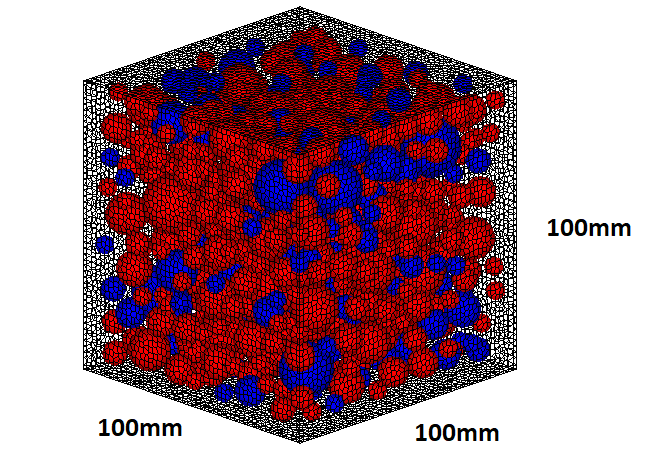
\includegraphics[width=.3\linewidth]{Files/Aggregate/A30P75.png}
  \caption{30\% Coarse Aggregate}
  \label{fig:A30P75_model}
\end{figure}


%A30P75FIX

\begin{figure}[ht]
\centering
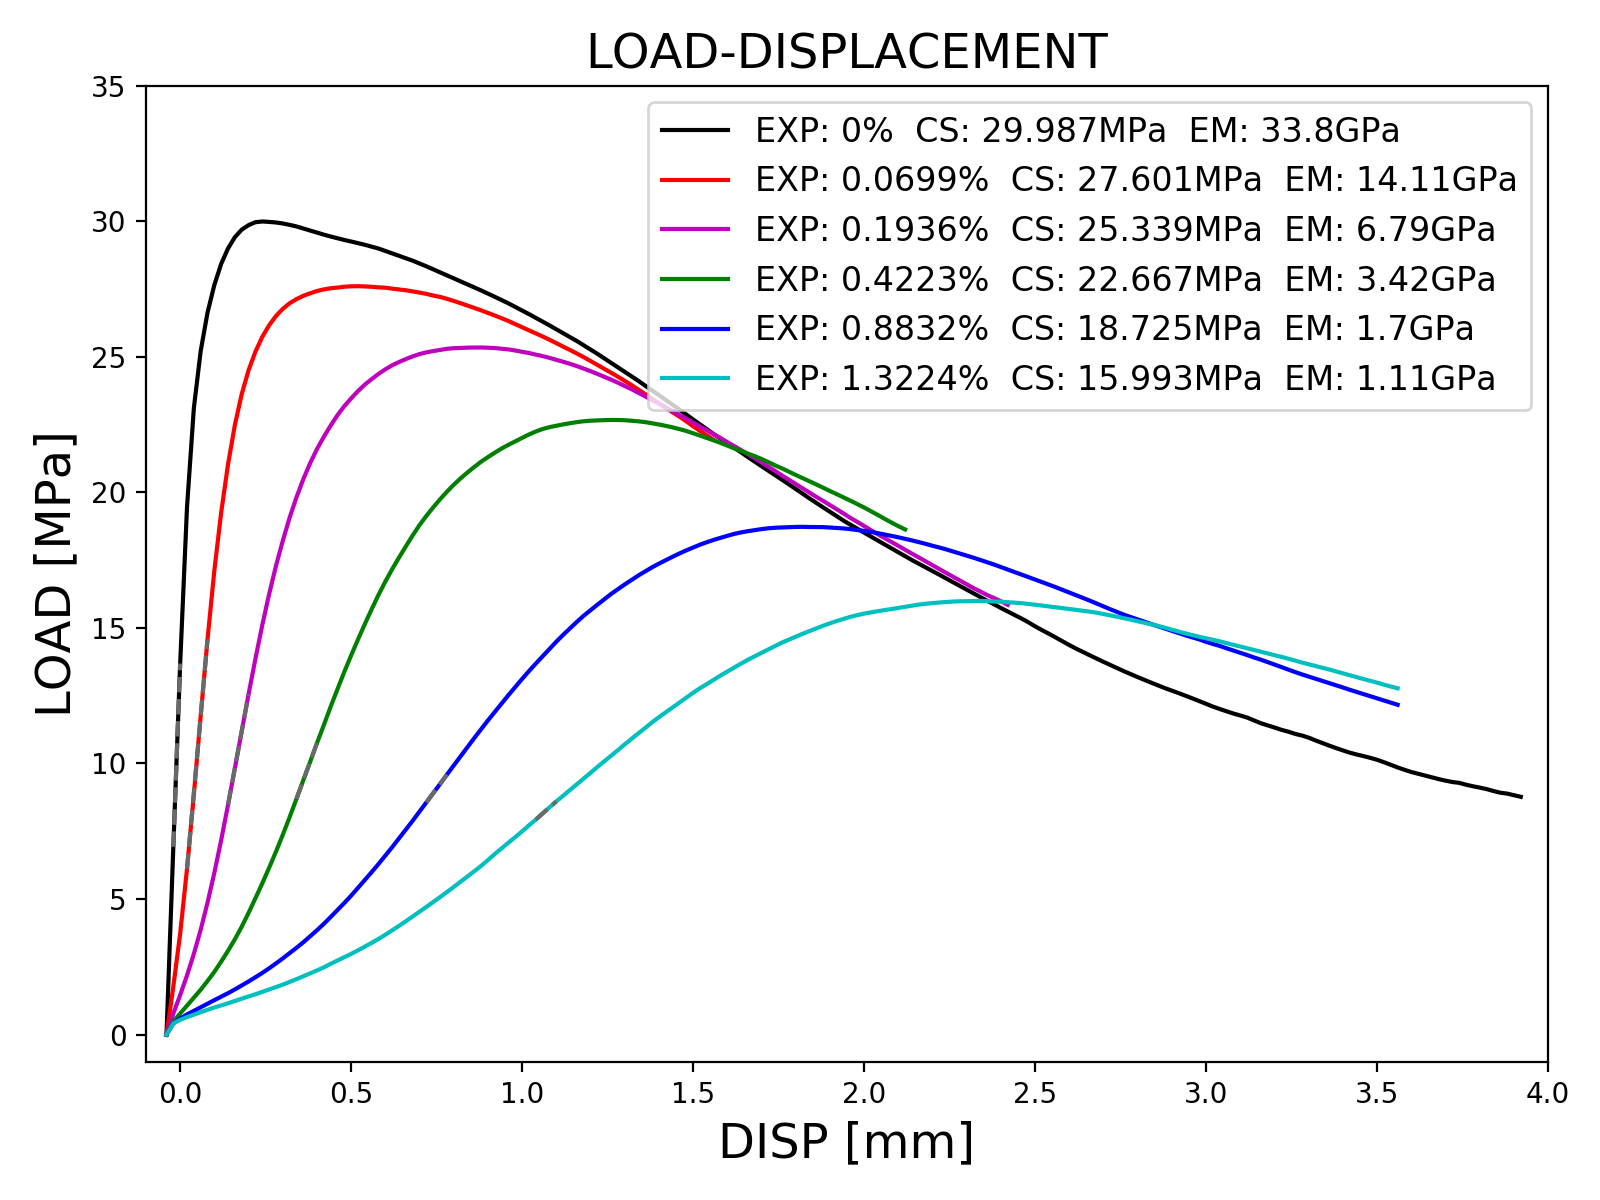
\includegraphics[width=.8\linewidth]{Files/exp_3D/ASR/S13A30P75FIX-LOAD-DISPLACEMENT.png}
  \caption{A30 P75 Fix Load-Displacement}
  \label{fig:A30P75FIX_LD}
\end{figure}




%A30P75FREE

\begin{figure}[ht!]
\centering
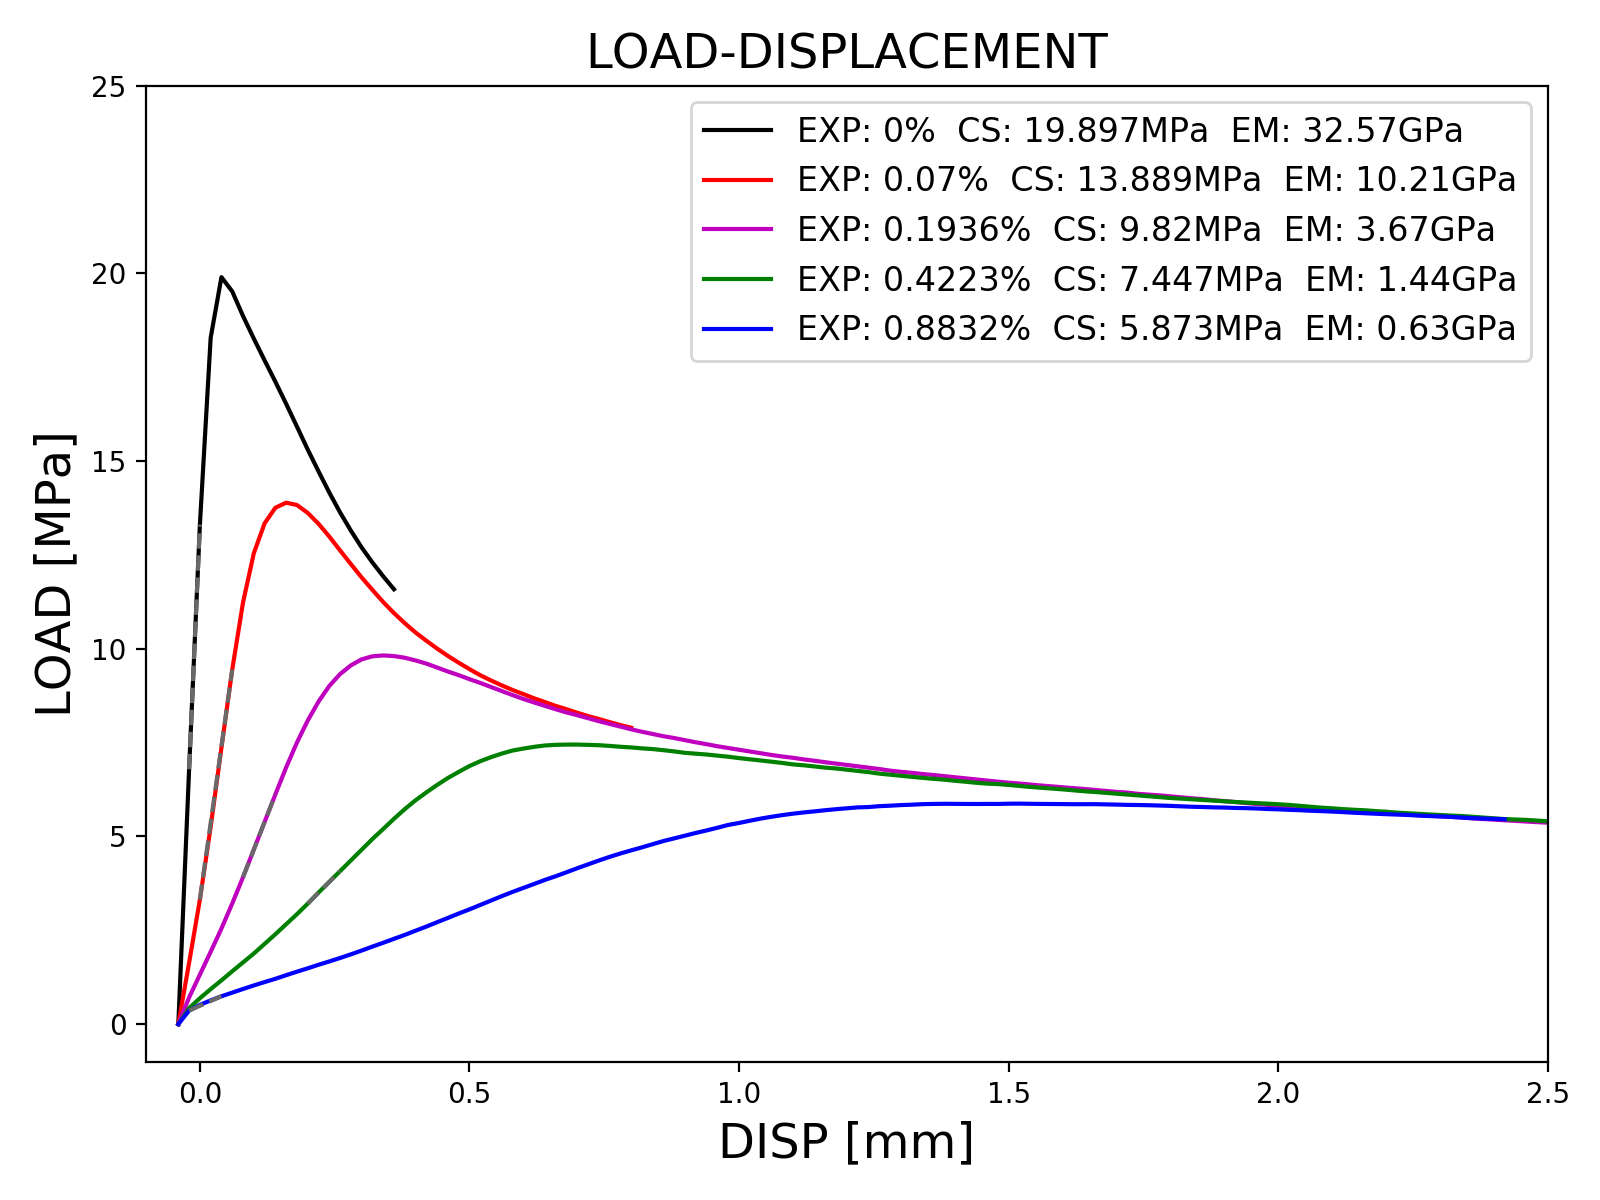
\includegraphics[width=.8\linewidth]{Files/exp_3D/ASR/S13A30P75FREE-LOAD-DISPLACEMENT.png}
  \caption{A30 P75 Free Load-Displacement}
  \label{fig:A30P75FREE_LD}
\end{figure}

\begin{table}[ht!]
\centering
\begin{tabular}{ ||p{2cm}|p{2cm}|p{2cm}|p{3cm}|p{3cm}|| }
 \hline
  Initial Strain (Each Step) & Expanding Steps & Final Expansion [\%] & Maximum Compressive Strength in Fix Loading Condition [MPa] & Maximum Compressive Strength in Free Loading Condition [MPa]\\ [0.5ex]
 \hline\hline
  0 & 0 & 0 & 29.987 & 19.897\\
  0.0002 & 20 & 0.0699 & 27.601 & 13.889\\
  0.0005 & 20 & 0.1936 & 25.339 & 9.8203\\
  0.001 & 20 & 0.4223 & 22.667 & 7.4466\\
  0.002 & 20 & 0.8832 & 18.725 & 5.8732 \\
  0.003 & 20 & 1.3224 & 15.993 &\\

 \hline
\end{tabular}
\caption{One Dimensional Expansion Ratio in Single ASR Model Simulation}
\label{table:ASR_30_EXP}
\end{table}

From the Figure \ref{fig:A30P75FIX_LD} and Figure \ref{fig:A30P75FREE_LD} it can be seen that with the increasing of given initial strain in each step, its global expansion ratio also increasing, and both maximum compressive strength in fix boundary condition and free boundary condition gradually decrease.




%A30P25FIX
\begin{figure}[ht]
\centering
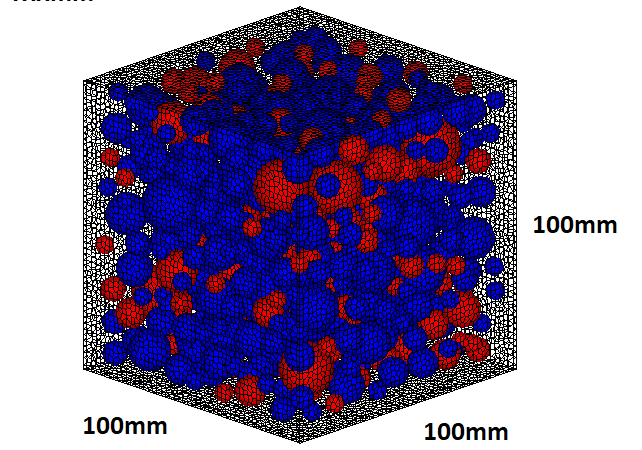
\includegraphics[width=.3\linewidth]{Files/Aggregate/A30P25.png}
  \caption{30\% Coarse Aggregate}
  \label{fig:A30P25_model}
\end{figure}

\begin{figure}[ht]
\centering
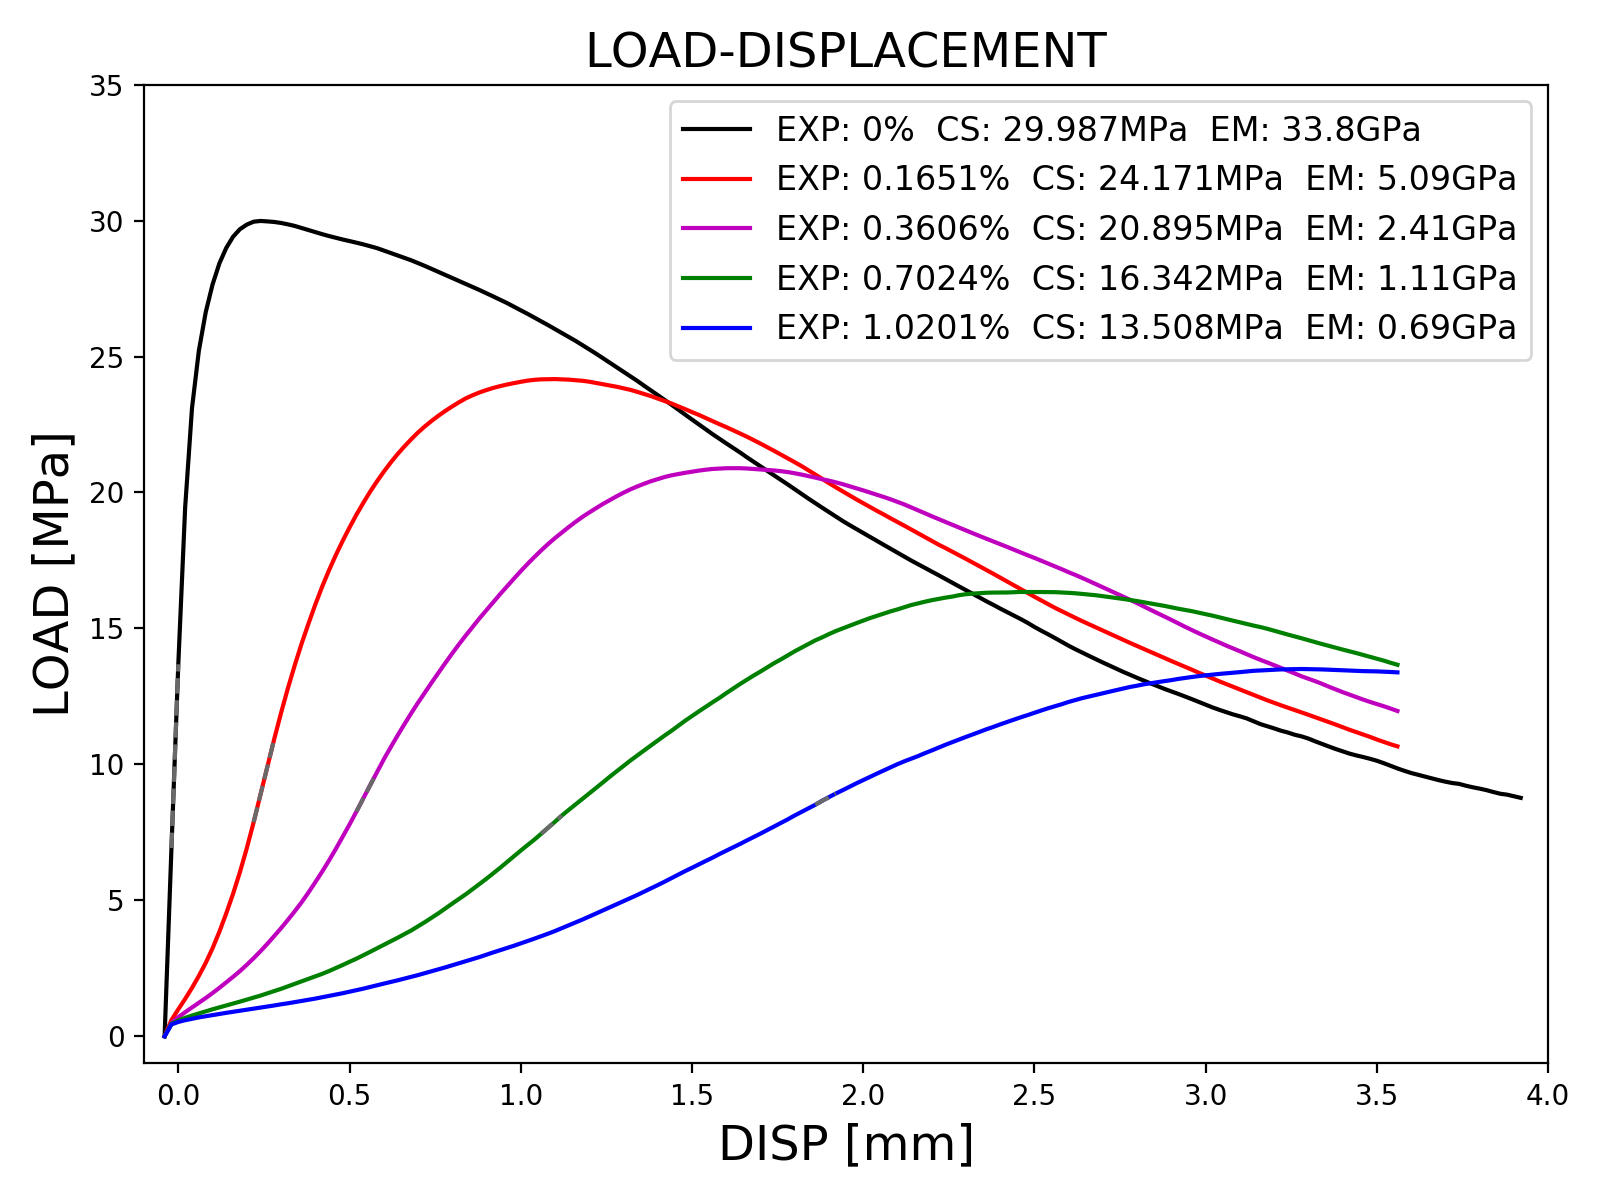
\includegraphics[width=.8\linewidth]{Files/exp_3D/ASR/S13A30P25FIX-LOAD-DISPLACEMENT.png}
  \caption{A30 P25 Fix Load-Displacement}
  \label{fig:A30P25FIX_LD}
\end{figure}

%A15P75FIX

\begin{figure}[ht]
\centering
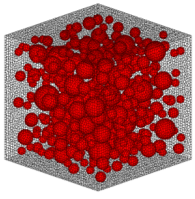
\includegraphics[width=.3\linewidth]{Files/Aggregate/A15.png}
  \caption{15\% Coarse Aggregate}
  \label{fig:A15P75_model}
\end{figure}

\begin{figure}[ht]
\centering
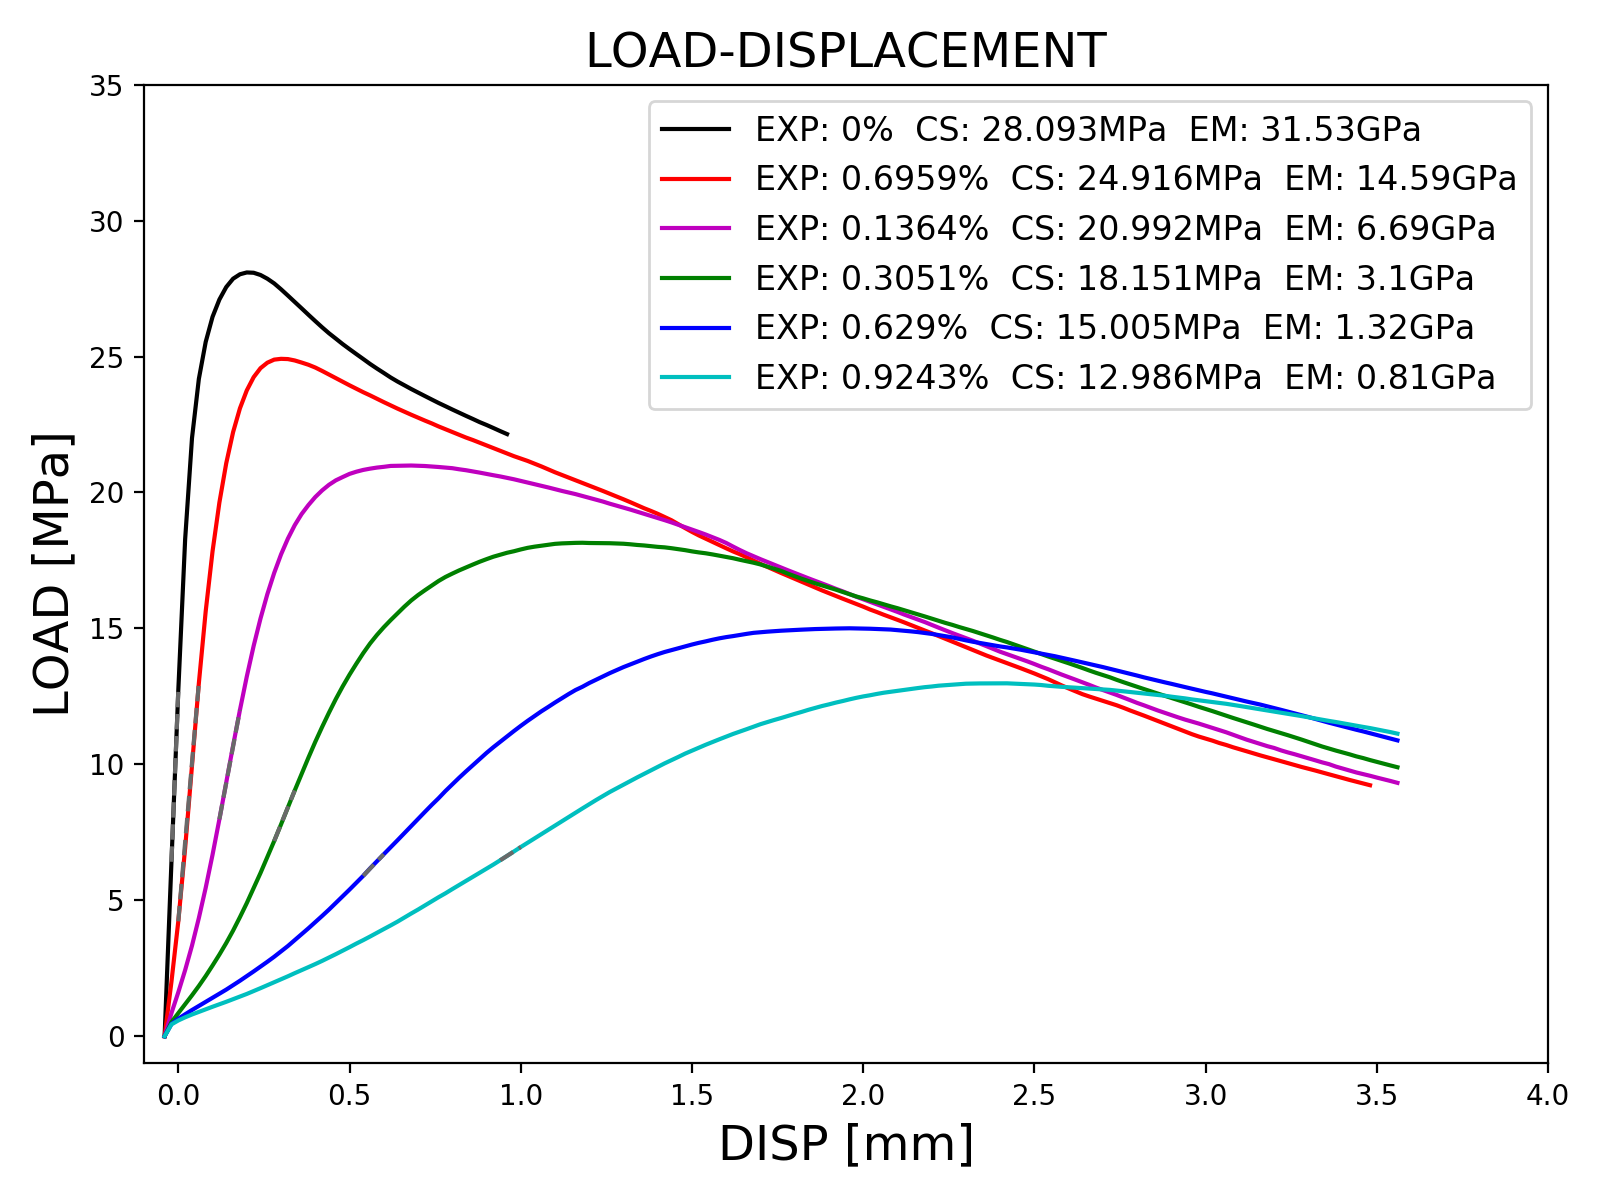
\includegraphics[width=.8\linewidth]{Files/exp_3D/ASR/S13A15P75FIX-LOAD-DISPLACEMENT.png}
  \caption{A15 P75 Fix Load-Displacement}
  \label{fig:A15P75FIX_LD}
\end{figure}
